\documentclass[11pt,twoside]{article}
\usepackage{asp2014}

\aspSuppressVolSlug
\resetcounters

\bibliographystyle{asp2014}

\markboth{Mueller et al.}{Qserv: A Distributed Petascale Database}

\begin{document}
%\ssindex{LSST}
%\ssindex{databases!petascale}
%\ssindex{observatories!ground-based!LSST}
%\ssindex{observatories!ground-based!Rubin}

\title{Qserv: A Distributed Petascale Database for the LSST Catalogs}

\author{Fritz~Mueller,$^1$ Igor~Gaponenko,$^1$ John~Gates,$^1$ Andrew~Hanushevsky,$^1$ Fabrice~Jammes,$^2$ Kian-Tat~Lim,$^1$ and Andrei~Salnikov$^1$}
\affil{$^1$SLAC National Accelerator Laboratory,  2575 Sand Hill Rd., Menlo Park, CA 94025, USA}
\affil{$^2$Universit\'e Clermont Auvergne, CNRS$/$IN2P3, Laboratoire de Physique de Clermont, F-63000 Clermont-Ferrand, France}
\paperauthor{Fritz~Mueller}{}{0000-0002-7061-4644}{SLAC National Accelerator Laboratory}{}{Menlo Park}{CA}{94025}{USA}
\paperauthor{Igor~Gaponenko}{}{}{SLAC National Accelerator Laboratory}{}{Menlo Park}{CA}{94025}{USA}
\paperauthor{John~Gates}{}{}{SLAC National Accelerator Laboratory}{}{Menlo Park}{CA}{94025}{USA}
\paperauthor{Andrew~Hanushevsky}{}{}{SLAC National Accelerator Laboratory}{}{Menlo Park}{CA}{94025}{USA}
\paperauthor{Fabrice~Jammes}{}{}{Universit\'e Clermont Auvergne}{}{Laboratoire de Physique de Clermont}{F-63000}{Clermont-Ferrand}{France}
\paperauthor{Kian-Tat~Lim}{}{0000-0002-6338-6516}{SLAC National Accelerator Laboratory}{}{Menlo Park}{CA}{94025}{USA}
\paperauthor{Andrei~Salnikov}{}{0000-0002-3623-0161}{SLAC National Accelerator Laboratory}{}{Menlo Park}{CA}{94025}{USA}
% Yes they said to have these index commands commented out.
%\aindex{Mueller,~F.}
%\aindex{Gaponenko,~I.}
%\aindex{Gates,~J.}
%\aindex{Hanushevsky,~A.}
%\aindex{Jammes,~F.}
%\aindex{Lim,~K.~T.}
%\aindex{Salnikov,~A.}

\begin{abstract}
Qserv is a distributed, shared-nothing, SQL database system being developed by the Vera Rubin Observatory to
host the multi-petabyte astronomical catalogs that will be produced by the LSST survey.  Here we sketch the
basic design and operating principles of Qserv, and provide some updates on recent developments.
\end{abstract}

\section{Introduction}

The Legacy Survey of Space and Time \citep{2019ApJ...873..111I} is a "deep fast wide" optical and near-IR
survey of half the sky in \emph{ugrizy} bands to \emph{r} 27.5 (36\,nJy) based on 825 visits over a 10-year
period, to be carried out by the Vera C.\ Rubin Observatory in Chile.

The astronomical catalogs to be produced by the survey are notionally described in \citet{LSE-163}, and the
corresponding database schema is described in \citet{LDM-153}.  By the 10th year of the survey, the catalog
database is expected to run to approximately 60 trillion rows, requiring more than 10 petabytes of storage
before considerations for replication, indices, or other overheads.

At the outset of construction, the project could not identify a mature database product capable of operating
at these scales while also meeting project requirements for robust spherical geometry, predictable query
response under heavy concurrent load, platform/hardware affordability, and open source licensing.  The Rubin
Observatory thus embarked on the design and implementation of Qserv.

\section{The Qserv Approach}

The evolution and progress of Qserv has been previously reported in \citet{2006SPIE.6270E..0RB},
\citet{2011Wang:2011:QDS:2063348.2063364}, and \citet{LDM-135}.  Qserv's principal design elements are as
follows:

\subsection{Distributed and Parallel}

Qserv is designed as a parallel database, where catalog data is spatially partitioned and distributed
uniformly over a collection of shared-nothing back-end nodes.  Queries are handled in a "map/reduce" paradigm:
after arriving at a SQL proxy, queries are analyzed for spatial coverage and rewritten into a collection of
supporting partial queries which are then distributed to involved back-end nodes for execution ("map" phase).
The results of these partial queries are subsequently returned to the proxy node where they are aggregated and
any necessary summary statistics computed ("reduce" phase). Results are then returned to the user.

\subsection{Partitioning and Replication}

\begin{figure}[t]
  $\vcenter{\hbox{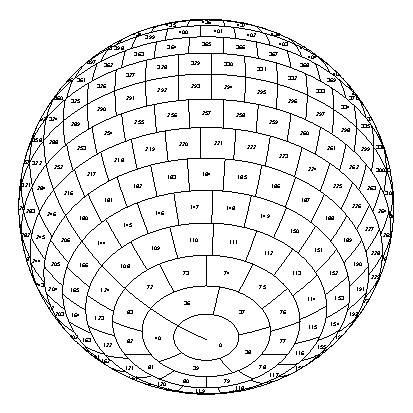
\includegraphics[width=0.48\textwidth]{C15_f1.eps}}}$
  \hfill
  $\vcenter{\hbox{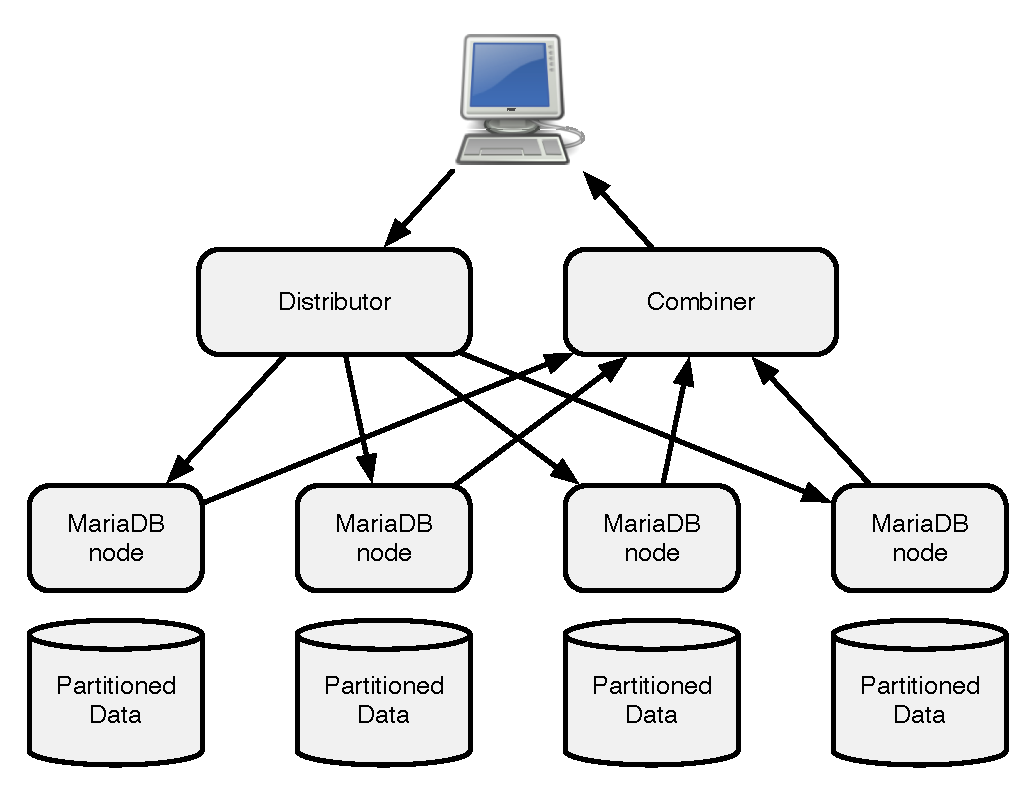
\includegraphics[width=0.48\textwidth]{C15_f2.eps}}}$
  \caption{[Left] Qserv partitioning scheme: rings of declination plus polar caps; roughly equi-area.
  [Right] Qserv "map/reduce" query processing.  Data is stationary on back-end nodes.}
\end{figure}

Qserv divides data into spatial partitions of roughly equal area.  Since partitions are small with respect to
higher-density areas of the survey and spread over back-end nodes using a non-area-based scheme,
density-differential-induced skew is averaged out among the nodes.

Qserv additionally stores a precomputed amount of overlapping data from spatially adjacent partitions
alongside each partition.  Using this data, spatial joins can be computed correctly within a preset distance
without needing data from other partitions that may be located on other nodes.

Data partitions are dynamically replicated across back-end nodes for resilience and high-availability.  If a
node becomes unavailable, Qserv is capable of transparently re-dispatching in-flight partial queries involving
partitions on that node toward other available partition replicas.  Partitions that become under-represented
are re-replicated and the cluster is periodically re-balanced in the background.  This same facility enables
the addition of nodes to a Qserv cluster or the draining of nodes for maintenance as online operations.

\subsection{Shared Scans}

Shared scans are a key component of the Qserv architecture and enable predictable query throughput on fixed
hardware under heavily concurrent loads.  As partial queries arrive at worker nodes, they are held and grouped
by involved partition(s).  Each node scans its local partitions in a cyclic and coordinated fashion. When a
scan visits a partition, its table backing files are locked into memory and all pending batched queries
involving that partition are executed.  The tables are then released and the scan proceeds to the next local
partition.

Multiple scan queues per node are supported to accommodate scans that execute at significantly different
speeds due to different amounts of I/O required.  In this way, time-consuming I/O intensive scans need not
hold up scans of other tables that could otherwise proceed more quickly.  Some capacity at each node is also
reserved to be able to quickly answer ad-hoc, non-scan queries to partitions on that node.

Partial queries may join a scan queue in any phase as they arrive at a node, and remain on the scan until all
involved partitions for that query on that node have been visited.

\subsection{Designed for Purpose}

Qserv, while broadly general purpose, has been specifically designed to meet the LSST catalog use-case. This
has allowed leverage of some significant simplifications to keep complexity low and to keep the project
feasible for a small development team.  For example: the LSST catalogs are to be released annually and are a
read-only product; thus Qserv does not need to address SQL UPDATE semantics nor does it need to encompass a
full transactional model.

Astronomical use demands robust spherical geometry within the database; Qserv has addressed this by providing
a library of precise spherical geometry UDFs which are made available for use of partial queries on the
back-end worker nodes.

Qserv has leveraged mature, open source, off-the-shelf components wherever possible; these include MariaDB,
the XRootD distributed file system, and Google protobufs.

Qserv is fully containerized and has a Kubernetes operator to facilitate deployment on Kubernetes, either
on-prem or in the commodity cloud.  We have found about a 15\% performance impact when running with network
storage on the Google cloud compared to running with locally attached storage on an on-prem cluster.

\section{Performance Targets and Sizing}

Performance targets for Qserv in the context of LSST have been established as follows.  Under a combined,
sustained load of 100 concurrent small ad-hoc queries and 50 concurrent full scans:
\[
{\renewcommand{\arraystretch}{1.5}\begin{array}{ll}
  \parbox{9cm}{Retrieve common attributes of an object, or all objects within a small area of the sky}
    & \mbox{< 10 seconds} \\
  \mbox{Scan entire sky (billions of objects)}
    & \mbox{$\approx{}$1 hour} \\
  \mbox{Deeper analysis (incl. object extended attribute BLOBs)}
    & \mbox{$\approx{}$8 hours} \\
  \mbox{Detection or forced photometry full scans}
    & \mbox{$\approx{}$12 hours} \\
\end{array}}
\]

Since Qserv is principally I/O limited, clusters are sized according to target full-scan times using the
following simple relations:

\[
    \frac{\text{table size(s)}}{\text{sustained I/O rate} * \text{workers}} = \text{target scan time}
\]

\[
    \frac{(\text{table size(s)} + \text{overlap} + \text{local indices}) * \text{replication}}
    {\text{workers}} = \text{local worker storage} \\
\]

For LSST, with consideration of the latest data sizing models \citep{DMTN-135}, this works out to a need for a
cluster of approximately 100 worker nodes for year 1 of the survey, peaking at approximately 450 worker nodes
in year 6, with approximately 45 TiB of local storage attached to each node.

\section{Conclusions}

Qserv's horizontal scaling capabilities have been demonstrated out to several hundreds of nodes, and the
system has been successful to date in meeting the construction and commissioning needs of the Rubin
Observatory serving pre-cursor datasets from clusters located at the National Center for Supercomputing
Applications and in the Google cloud.  Most recently this has included support for a community of several
hundred users as an integrated component of the Rubin Science Platform for Rubin Observatory's Data Preview
0.2 \citep{RTN-041}. Additional clusters are now being commissioned at each of the LSST international data
centers (USA, France, UK).  We hope the astronomical community may also find use for Qserv and its design
ideas beyond the LSST survey.

\acknowledgements This material or work is supported in part by the National Science Foundation through
Cooperative Agreement AST-1258333 and Cooperative Support Agreement AST1836783 managed by the Association of
Universities for Research in Astronomy (AURA), and the Department of Energy under Contract No.
DE-AC02-76SF00515 with the SLAC National Accelerator Laboratory managed by Stanford University.

\bibliography{C15}

\end{document}
